\section{Implementarea laboratorului 2 }

\subsection{Taskuri implementate}

\begin{itemize}
\item Realizeaza un simplu GUI calculator care suporta functiile de baza: +, -, /, *.
\item Realizeaza un simplu GUI calculator care suporta urmatoare functii: +, -, /, *, putere, radical, InversareSemn(+/-).

\item Realizeaza un simplu GUI calculator care suporta urmatoare functii: +, -, /, *, putere, radical, InversareSemn(+/-), operatii cu numere zecimale.

\item Divizarea proiectului in doua module - Interfata grafica(Modul GUI) si Modulul de baza(Core Module).

\end{itemize}

\subsection{Analiza lucrarii de laborator}

In lucrarea de laborator a fost realizat un calculator grafic ce realizeaza o serie de operatii matematice 
utilizind numere intregi si numere zecimale.
Codul sursa se gaseste pe repozitoriul github.

\subsection{Realizarea unui calculator GUI simplu}

Pentru realizarea calculatorului a fost folosit Visual Studio 2015 si limbajul de programare CSharp, 
deoarece este unul din cele mai potrivite si mai comode pentru realizarea acestui scop.
Visual Studio are implementata o interfata ce contine foarte multe elemnte care pot fi atasate 
ferestrelor prin metoda drag-and-drop, respectiv in acelasi timp generindu-se si o parte din 
metoda fiecarui element cit si proprietati si tratare de evenimente.

\begin{figure}[!ht]
                     \centering
                     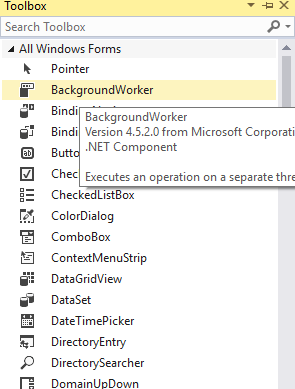
\includegraphics[scale = 0.6]{toolbox}
                     \caption{Toolboxul din Visual Studio, \cite{ImRef}}
                     \label{Im_label}
                \end{figure}


Cum am specificat mai sus Visual Studio este foarte potrivit pentru a separa partea grafica
a aplicatiei de cea logica.Respectiv avem mai jos interfata grafica a aplicatiei.

\begin{figure}[!ht]
                     \centering
                     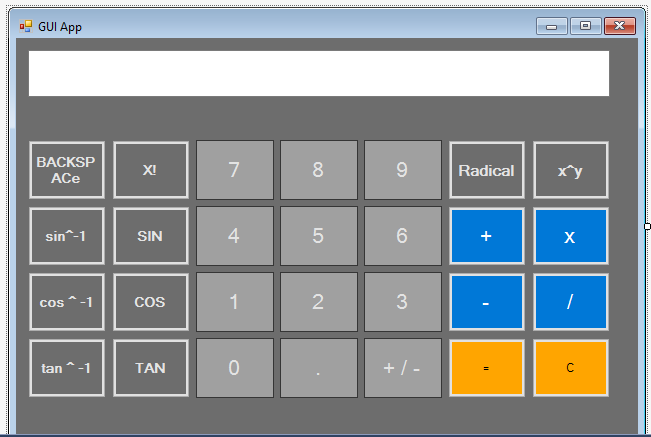
\includegraphics[scale = 0.6]{interface}
                     \caption{Interfata aplicatiei, \cite{ImRef}}
                     \label{Im_label}
                \end{figure}

Iar partea logica nu va trebui modificata in cazul unor schimbari de desing sau de restyle,
ea se contine in fisierul Form1.cs

\begin{figure}[!ht]
                     \centering
                     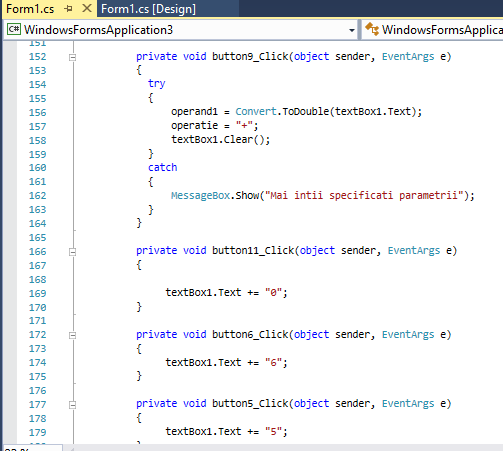
\includegraphics[scale = 0.6]{logic}
                     \caption{Partea logica a aplicatiei, \cite{ImRef}}
                     \label{Im_label}
                \end{figure}
                
La realizarea aplicatiei sa tinut cont si de anumite anomalii de executie, cum ar fi tastarea anumitor butoane 
inaintea suplinirii cu parametri, sau executia unei operatii nule, asa  ca sa luat decizia implementarii 
unor tipuri de handlere ale acestor evenimente, respectiv afisare unor mesaje de pre-intimpinare  
a utilizatorului, astfel utilizatorul va primi un MessageBox cu mesajul de eroare respectiv.


\begin{figure}[!ht]
                     \centering
                     \includegraphics[scale = 1]{Error}
                     \caption{Mesaj de pre-intimpinare a utilizatorului, \cite{ImRef}}
                     \label{Im_label}
                \end{figure}
               


\clearpage